\documentclass[10pt,aspectratio=169]{beamer}

\usefonttheme{professionalfonts}
\setbeamertemplate{navigation symbols}{}
\setbeamertemplate{blocks}[default]

% Uncomment one of these for presenter mode:
% \usepackage{pgfpages}
% \setbeameroption{show notes on second screen=right}
% \setbeameroption{show notes}

\usepackage{booktabs}
\usepackage{amsmath}
\usepackage{amssymb}
\usepackage{xcolor}
\usepackage{tikz}
\usetikzlibrary{arrows.meta, positioning}
\usepackage{graphicx}
\usepackage{array}
\usepackage[round,authoryear]{natbib}

\definecolor{ink}{RGB}{20,24,31}
\definecolor{muted}{RGB}{91,99,112}
\definecolor{rulegray}{RGB}{196,202,211}
\definecolor{accent}{RGB}{29,78,137}
\definecolor{softgray}{RGB}{246,247,249}

\setbeamercolor{normal text}{fg=ink,bg=white}
\setbeamercolor{structure}{fg=accent}
\setbeamercolor{frametitle}{fg=ink,bg=white}
\setbeamercolor{title}{fg=ink}
\setbeamercolor{subtitle}{fg=muted}
\setbeamercolor{author}{fg=ink}
\setbeamercolor{institute}{fg=muted}
\setbeamercolor{date}{fg=muted}
\setbeamerfont{title}{size=\Large,series=\bfseries}
\setbeamerfont{subtitle}{size=\normalsize}
\setbeamerfont{frametitle}{size=\large,series=\bfseries}
\setbeamerfont{footline}{size=\scriptsize}
\setbeamerfont{caption}{size=\scriptsize}

\setbeamertemplate{frametitle}{%
  \vspace{0.35em}
  \insertframetitle\par
  \vspace{0.22em}
  {\color{rulegray}\rule{\linewidth}{0.35pt}}
}

\setbeamertemplate{footline}{%
  \leavevmode%
  \hbox{%
    \begin{beamercolorbox}[wd=.72\paperwidth,ht=2.5ex,dp=1ex,leftskip=.55cm]{footline}%
      \textcolor{muted}{Functional forecasting of Turkish load curves}
    \end{beamercolorbox}%
    \begin{beamercolorbox}[wd=.28\paperwidth,ht=2.5ex,dp=1ex,rightskip=.55cm plus1fil]{footline}%
      \hfill\textcolor{muted}{\insertframenumber/\inserttotalframenumber}
    \end{beamercolorbox}%
  }%
}

\setlength{\tabcolsep}{5pt}
\renewcommand{\arraystretch}{1.18}
\newcommand{\claim}[1]{\vspace{0.15em}{\small\textbf{#1}}\vspace{0.35em}}
\newcommand{\source}[1]{\vspace{0.25em}{\scriptsize\textcolor{muted}{#1}}}
\newcommand{\modelmain}{K=2 FPCA--VAR score model}
\newcommand{\teias}{TE\.{I}A\c{S}}

\title{Functional Forecasting of Turkish Electricity Load Curves}
\subtitle{Thesis proposal v3}
\author{Zeynep Bozoklu}
\institute{PhD proposal}
\date{June 2026}

\begin{document}

% ============================================================
% SLIDE 1
% ============================================================
\begin{frame}[plain]
  \vspace{0.75cm}
  {\usebeamerfont{title}\inserttitle\par}
  \vspace{0.15cm}
  {\usebeamerfont{subtitle}\textcolor{muted}{\insertsubtitle}\par}
  \vspace{0.75cm}

  \begin{tabular}{@{}ll@{}}
    \toprule
    Object & Daily curve $Y_d(h),\ h=0,\ldots,23$ \\
    Main model & \modelmain{} with holiday, load-shape, derivative features \\
    Benchmark & Official day-ahead forecast published by \teias{} / EPIAS \\
    Evaluation & Rolling origin, 2023--2025, 1,096 days, 26,304 hourly errors \\
    Test & Diebold--Mariano, pooled and hour-by-hour \\
    \bottomrule
  \end{tabular}

  \vfill
  \begin{tabular}{@{}ll@{}}
    \textbf{Zeynep Bozoklu} & \textcolor{muted}{\insertinstitute} \\
  \end{tabular}
  \note{Open with the empirical object and the evaluation discipline. The thesis asks whether a transparent functional model can improve the official day-ahead benchmark. The main result is the K=2 FPCA--VAR score model: MAE 980, 19.2 percent better than the official forecast, with a pooled DM p-value near 10^{-163}.}
\end{frame}

% ============================================================
% SLIDE 2
% ============================================================
\begin{frame}{Forecasting Question}
  \begin{minipage}[t]{0.54\textwidth}
      \vspace{0pt}\raggedright
      \claim{Operational question}
      Can a functional statistical model forecast tomorrow's full 24-hour load
      profile more accurately than the official benchmark, using only information
      available before the target day?

      \vspace{0.75em}
      \claim{Descriptive starting point}
      The official forecast is systematically below realized load over the
      evaluation window. The proposed model reduces the average hourly bias by
      roughly four-fifths.
  \end{minipage}\hfill
  \begin{minipage}[t]{0.38\textwidth}
      \vspace{0pt}\raggedright
      \small
      \begin{tabular}{lrr}
        \toprule
        Year & Official bias & Main model bias \\
             & MWh/hour & MWh/hour \\
        \midrule
        2023 & 344 & 176 \\
        2024 & 585 & 34 \\
        2025 & 472 & 98 \\
        \midrule
        Average & \textbf{467} & \textbf{103} \\
        \bottomrule
      \end{tabular}
      \source{Positive bias: actual $>$ forecast.}
  \end{minipage}
  \note{Keep the framing empirical and operational. The official forecast is the correct benchmark because it is observed on the same days and hours as the target. Bias is not the only metric, but it motivates the forecasting exercise.}
\end{frame}

% ============================================================
% SLIDE 3
% ============================================================
\begin{frame}{Forecasting Object: One Curve, Not 24 Unrelated Targets}
  \begin{columns}[T,onlytextwidth]
    \begin{column}{0.63\textwidth}
      \includegraphics[width=\linewidth]{../output/figs/fda_mean_actual_forecast_all.png}
    \end{column}
    \begin{column}{0.34\textwidth}
      \[
        Y_d = \{Y_d(h): h=0,\ldots,23\}
      \]
      \small
      \begin{itemize}
        \item Hourly observations form a coherent daily trajectory.
        \item Level, peak contrast, and ramp speed are curve-level features.
        \item FDA reduces a 24-dimensional problem to a small number of scores.
      \end{itemize}
      \source{Solid = actual mean curve; dashed = official mean forecast.}
    \end{column}
  \end{columns}
  \note{The important conceptual move is to treat the day as a function. The hourly values are strongly ordered and shape-constrained. This justifies B-spline smoothing, FPCA compression, and reconstruction from predicted scores.}
\end{frame}

% ============================================================
% SLIDE 4
% ============================================================
\begin{frame}{Research Design}
  \begin{center}
  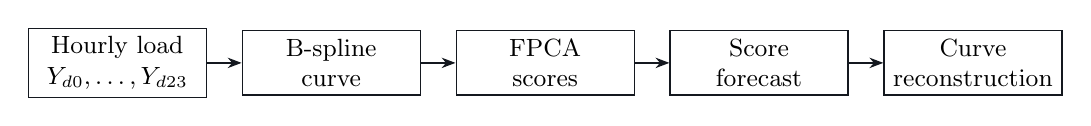
\begin{tikzpicture}[
    node distance=0.32cm and 0.44cm,
    box/.style={rectangle, draw=ink, fill=white, line width=0.45pt,
                text width=2.05cm, align=center, font=\small,
                minimum height=0.78cm, inner sep=3pt},
    arr/.style={-Stealth, line width=0.45pt, draw=ink}
  ]
    \node[box] (raw) {Hourly load\\$Y_{d0},\ldots,Y_{d23}$};
    \node[box, right=of raw] (spline) {B-spline\\curve};
    \node[box, right=of spline] (fpca) {FPCA\\scores};
    \node[box, right=of fpca] (score) {Score\\forecast};
    \node[box, right=of score] (recon) {Curve\\reconstruction};

    \draw[arr] (raw) -- (spline);
    \draw[arr] (spline) -- (fpca);
    \draw[arr] (fpca) -- (score);
    \draw[arr] (score) -- (recon);
  \end{tikzpicture}
  \end{center}

  \vspace{0.6em}
  \begin{columns}[T,onlytextwidth]
    \begin{column}{0.48\textwidth}
      \small
      \[
        Y_d(h) \approx \mu(h) + \sum_{k=1}^{K}\xi_{dk}\phi_k(h)
      \]
      \[
        \hat{Y}_d(h) =
        \hat{\mu}(h)+\sum_{k=1}^{K}\hat{\xi}_{dk}\hat{\phi}_k(h)
      \]
    \end{column}
    \begin{column}{0.48\textwidth}
      \small
      Design principles:
      \begin{itemize}
        \item low-dimensional representation;
        \item expanding-window estimation;
        \item official forecast as external benchmark;
        \item formal forecast-accuracy testing.
      \end{itemize}
    \end{column}
  \end{columns}
  \note{Use this as the map for the rest of the talk. The model does not forecast 24 hours separately. It forecasts the FPCA scores and then reconstructs the entire curve.}
\end{frame}

% ============================================================
% SLIDE 5
% ============================================================
\begin{frame}{FPCA Compression and Stability}
  \begin{columns}[T,onlytextwidth]
    \begin{column}{0.58\textwidth}
      \includegraphics[width=\linewidth]{../output/figs/eigenfunction_shape_comparison.png}
    \end{column}
    \begin{column}{0.38\textwidth}
      \small
      \begin{tabular}{rrr}
        \toprule
        FPC & Variance & Cumulative \\
        \midrule
        1 & 93.4\% & 93.4\% \\
        2 & 3.9\% & 97.3\% \\
        3 & 1.1\% & 98.4\% \\
        4 & 1.0\% & 99.4\% \\
        \bottomrule
      \end{tabular}

      \vspace{0.75em}
      \small
      \begin{tabular}{@{}ll@{}}
        FPC 1 & level \\
        FPC 2 & shape contrast \\
        Stability & IP $>0.99$ \\
        Robustness & $K=4$ unchanged \\
      \end{tabular}
    \end{column}
  \end{columns}
  \note{The central technical fact is that two components retain 97.3 percent of variation. This makes the score forecast interpretable. FPC 1 is mostly a level shift. FPC 2 changes the shape contrast across the day. The basis is stable across sub-periods, so the representation is not an artifact of a single window.}
\end{frame}

% ============================================================
% SLIDE 6
% ============================================================
\begin{frame}{Score Forecasting Model}
  \begin{columns}[T,onlytextwidth]
    \begin{column}{0.50\textwidth}
      \[
        \xi_d
        = a + A_1\xi_{d-1} + A_7\xi_{d-7} + Bz_d + u_d
      \]
      \[
        z_d \in \mathcal{F}_{d-1}
      \]
      \small
      Estimated equation-by-equation by OLS. The target is the score vector,
      not an individual hour.
    \end{column}
    \begin{column}{0.46\textwidth}
      \small
      \begin{tabular}{@{}l>{\raggedright\arraybackslash}p{0.58\linewidth}@{}}
        \toprule
        Block & Variables \\
        \midrule
        Score dynamics & lag 1, lag 7 \\
        Calendar & weekend, annual sine/cosine \\
        Holiday & public holidays, Eid, bridge days \\
        Load shape & lagged mean, peak, range \\
        Rolling history & 7-day, 28-day averages \\
        Derivative & ramp summaries, slope volatility \\
        \bottomrule
      \end{tabular}
    \end{column}
  \end{columns}
  \vspace{0.6em}
  \source{$\mathcal{F}_{d-1}$ denotes the information set before target day $d$; lagged curves are treated as known.}
  \note{Clarify terminology: FPCA--OLS means FPCA scores are forecast by an OLS score equation. It is not 24 separate hourly OLS models. The derivative block comes from differentiating the smoothed curve and summarising ramp behavior.}
\end{frame}

% ============================================================
% SLIDE 7
% ============================================================
\begin{frame}{Rolling-Origin Evaluation and DM Test}
  \begin{columns}[T,onlytextwidth]
    \begin{column}{0.48\textwidth}
      \small
      For each target day $d$:
      \[
        \{1,\ldots,d-1\}
        \quad\Longrightarrow\quad
        \hat{Y}_d(0{:}23)
      \]

      \vspace{0.6em}
      Metrics pooled over all target days and hours:
      \[
        \text{MAE},\qquad \text{MAPE}
      \]
    \end{column}
    \begin{column}{0.48\textwidth}
      \small
      Diebold--Mariano loss differential:
      \[
        \Delta_t =
        |e_t^{\text{model}}|-|e_t^{\text{official}}|
      \]
      \[
        H_1:\mathbb{E}[\Delta_t] < 0
      \]
      HAC variance and Harvey--Leybourne--Newbold correction.

      \vspace{0.4em}
      Same test is also run separately for each hour $h$:
      \[
        \Delta_{d,h}=|e_{d,h}^{m}|-|e_{d,h}^{o}|.
      \]
    \end{column}
  \end{columns}
  \note{This slide answers the DM question directly. The pooled DM test gives an overall accuracy test across 26,304 hourly errors. The hour-by-hour DM tests repeat the same loss-differential logic for each fixed hour, so they identify where the improvement is statistically reliable.}
\end{frame}

% ============================================================
% SLIDE 8
% ============================================================
\begin{frame}{Main Empirical Result}
  \begin{center}
  \small
  \begin{tabular}{p{0.43\textwidth}rrrc}
    \toprule
    Model & MAE & MAPE & Gain vs official & DM \\
    \midrule
    Seasonal naive $Y_{d-7}$ & 1912 & 5.13\% & $-57.6\%$ & -- \\
    Official \teias{} forecast & 1214 & 3.15\% & ref. & -- \\
    \midrule
    FPCA--VAR scores only & 1443 & 3.76\% & $-18.9\%$ & worse \\
    $+$ calendar / ramp & 1238 & 3.26\% & $-2.1\%$ & n.s. \\
    $+$ holiday / load-shape & 1001 & 2.63\% & $+17.5\%$ & *** \\
    \textbf{$+$ derivative features} & \textbf{980} & \textbf{2.56\%} & \textbf{$+19.2\%$} & \textbf{***} \\
    \midrule
    Residual second step & 653 & 1.70\% & $+46.2\%$ & *** \\
    \bottomrule
  \end{tabular}
  \end{center}
  \source{Evaluation: 2023--2025. Main model pooled DM statistic $=-27.4$, $p\approx 1.3\times10^{-163}$. MAE in MWh/hour.}
  \note{Read this as a specification path, not as a list of unrelated models. Pure score dynamics are not enough. Holiday and load-shape variables create the large jump, and derivative features produce the final main model. The residual row is a second-step extension, not the baseline thesis model.}
\end{frame}

% ============================================================
% SLIDE 9
% ============================================================
\begin{frame}{Hourly Diagnostics for the Main Model}
  \begin{minipage}[t]{0.61\textwidth}
    \vspace{0pt}
    \includegraphics[width=\linewidth]{../output/figs/thesis_v3_main_gain_by_hour.png}
  \end{minipage}\hfill
  \begin{minipage}[t]{0.33\textwidth}
      \vspace{0pt}
      \small
      \begin{tabular}{@{}lr@{}}
        \toprule
        Diagnostic & Count \\
        \midrule
        Lower MAE & 19 / 24 \\
        DM-significant & 18 / 24 \\
        Weak window & 6--9 \\
        Strong gains & 0--5, 10--17 \\
        \bottomrule
      \end{tabular}

      \vspace{0.65em}
      Positive bars indicate lower MAE than the official benchmark. The table
      distinguishes raw wins from statistically significant wins.
  \end{minipage}
  \note{This slide prevents overclaiming. The main FPCA--VAR model wins most hours, but not every hour. It has lower MAE at 19 of 24 hours and DM-significant gains at 18 of 24 hours. The weak window is concentrated around the morning transition.}
\end{frame}

% ============================================================
% SLIDE 10
% ============================================================
\begin{frame}{Residual Second Step}
  \begin{columns}[T,onlytextwidth]
    \begin{column}{0.56\textwidth}
      \includegraphics[width=\linewidth]{../output/figs/acf_base_vs_correction.png}
    \end{column}
    \begin{column}{0.40\textwidth}
      \small
      Base-model residuals are serially structured:
      \[
        r_d(h)=Y_d(h)-\hat{Y}^{\text{base}}_d(h)
      \]
      Correction:
      \[
        \hat{Y}^{\text{res}}_d(h)
        =
        \hat{Y}^{\text{base}}_d(h)
        + \lambda_d\hat{r}_d(h)
      \]
      \[
        \lambda_d \text{ chosen by rolling-origin CV}
      \]
      using pre-$d$ data only.

      \vspace{0.5em}
      Result: MAE 653, MAPE 1.70\%, gain $+46.2\%$, lower MAE at 24/24 hours.
    \end{column}
  \end{columns}
  \note{The residual step is evidence that the baseline errors contain predictable serial structure. It uses only past residual curves and rolling-origin cross-validation. This makes it a defensible extension rather than a post-hoc fit on the evaluation errors.}
\end{frame}

% ============================================================
% SLIDE 11
% ============================================================
\begin{frame}{Random Forest Benchmark}
  \begin{minipage}[t]{0.53\textwidth}
    \vspace{0pt}
    \includegraphics[width=\linewidth]{../output/figs/thesis_v3_rf_benchmark_by_hour.png}
  \end{minipage}\hfill
  \begin{minipage}[t]{0.41\textwidth}
      \vspace{0pt}
      \small
      Benchmark sample: 2023, 8,760 hourly forecasts.

      \vspace{0.45em}
      \begin{tabular}{@{}lrrc@{}}
        \toprule
        Model & MAE & Gain & DM \\
        \midrule
        Official & 1052 & ref. & -- \\
        FPCA score & 910 & $+13.5\%$ & *** \\
        Direct RF & 718 & $+31.8\%$ & *** \\
        \bottomrule
      \end{tabular}

      \vspace{0.55em}
      Direct RF predicts each hour directly and bypasses FPCA. It has lower MAE
      at 24/24 hours on this sample; pairwise DM vs the FPCA--VAR score model:
      $p\approx1.2\times10^{-85}$.
  \end{minipage}
  \par\vspace{0.25em}
  {\scriptsize\textcolor{muted}{FPCA score = main K=2 model without residual correction, restricted to the same 2023 benchmark sample.}}
  \note{Be explicit that this is a different model class and a shorter sample. It does not replace the main 2023--2025 thesis result. It shows that a direct nonlinear hourly benchmark is very strong, and it should be reported honestly.}
\end{frame}

% ============================================================
% SLIDE 12
% ============================================================
\begin{frame}{What Each Comparison Answers}
  \small
  \begin{tabular}{p{0.28\textwidth}p{0.33\textwidth}p{0.30\textwidth}}
    \toprule
    Comparison & Statistical question & Interpretation \\
    \midrule
    Main FPCA--VAR vs official &
    Does a transparent functional score model improve the operational benchmark? &
    Yes: $+19.2\%$ MAE, pooled DM $p\approx10^{-163}$. \\
    \addlinespace
    Residual step vs official &
    Are base-model errors predictably autocorrelated? &
    Yes: residual correction wins at all hours. \\
    \addlinespace
    Direct RF vs official &
    How strong is a direct nonlinear hourly benchmark on the 2023 sample? &
    Very strong: $+31.8\%$ MAE, DM significant. \\
    \addlinespace
    Direct RF vs FPCA--VAR &
    Does the direct nonlinear benchmark beat the interpretable score model on the same 2023 sample? &
    Yes: pairwise DM $p\approx1.2\times10^{-85}$. \\
    \bottomrule
  \end{tabular}
  \vspace{0.8em}

  \claim{Thesis position}
  The FPCA--VAR model is the interpretable functional baseline; Direct RF is a
  serious benchmark that documents remaining nonlinear predictive structure.
  \note{This slide resolves possible confusion from the RF result. We are not hiding the RF result, and we are not pretending all models answer the same question. The main thesis contribution is interpretable functional forecasting with formal benchmarking. The RF result gives a stronger applied benchmark and motivates either a nonlinear extension or a clearly separated benchmark chapter.}
\end{frame}

% ============================================================
% SLIDE 13
% ============================================================
\begin{frame}{Contributions and Status}
  \small
  \begin{tabular}{p{0.31\textwidth}p{0.58\textwidth}}
    \toprule
    Contribution & Evidence in current draft \\
    \midrule
    Functional representation &
    B-spline curves; $K=2$ FPCA retains 97.3\%; stable eigenfunctions. \\
    Forecasting model &
    Expanding-window FPCA--VAR score model with predetermined feature blocks. \\
    Formal benchmark testing &
    Pooled and hour-specific Diebold--Mariano tests against the official forecast. \\
    Residual diagnostics &
    Autocorrelation motivates a no-lookahead residual second step. \\
    Nonlinear benchmark &
    Direct RF reported separately, with MAE and DM comparisons. \\
    \bottomrule
  \end{tabular}

  \vspace{0.8em}
  \begin{tabular}{@{}ll@{}}
    Done & empirical pipeline, main results, RF benchmark, DM diagnostics \\
    Open & systematic literature review, final write-up, scope decision on intervals \\
  \end{tabular}
  \note{This is the proposal close. It tells the committee what is already empirically established and what still has to be written or scoped. Keep it candid: the empirical core is strong, but literature positioning and final thesis framing remain active work.}
\end{frame}

% ============================================================
% SLIDE 14
% ============================================================
\begin{frame}{References}
  \footnotesize
  \begin{thebibliography}{99}

    \bibitem[Diebold and Mariano(1995)]{dm_1995}
    Diebold, F.X. and Mariano, R.S. (1995).
    Comparing predictive accuracy.
    \textit{Journal of Business \& Economic Statistics}, 13(3), 253--263.

    \bibitem[Harvey, Leybourne and Newbold(1997)]{hln_1997}
    Harvey, D., Leybourne, S. and Newbold, P. (1997).
    Testing the equality of prediction mean squared errors.
    \textit{International Journal of Forecasting}, 13(2), 281--291.

    \bibitem[Hyndman and Ullah(2007)]{hyndman_2007}
    Hyndman, R.J. and Ullah, M.S. (2007).
    Robust forecasting of mortality and fertility rates:
    a robust functional data approach.
    \textit{Computational Statistics \& Data Analysis}, 51(10), 4942--4956.

    \bibitem[Kokoszka and Reimherr(2017)]{kokoszka_2017}
    Kokoszka, P. and Reimherr, M. (2017).
    \textit{Introduction to Functional Data Analysis}. CRC Press.

    \bibitem[Xie and Hong(2016)]{xie_2016}
    Xie, J. and Hong, T. (2016).
    GEFCom2014 probabilistic electric load forecasting:
    an integrated solution with forecast combination and residual simulation.
    \textit{International Journal of Forecasting}, 32(3), 1012--1016.

  \end{thebibliography}
  \note{Use this slide only for questions. Diebold--Mariano and Harvey--Leybourne--Newbold support the testing framework. Kokoszka--Reimherr and Hyndman--Ullah support the functional forecasting framework. Xie--Hong is useful background for residual correction in load forecasting.}
\end{frame}

\end{document}
